\documentclass[12pt,a4paper]{report}

\usepackage[portuguese]{babel}
\usepackage{hyphenat}
\usepackage{amsmath}
\usepackage{amsfonts}
\usepackage{amssymb}
\usepackage{amsthm}
\usepackage{graphicx}
\usepackage{makeidx}
\usepackage{enumerate}
\usepackage[square,sort,comma,numbers]{natbib}
\usepackage[left=1.25in,right=1in,top=1in,bottom=1in]{geometry}
\usepackage{setspace}
\usepackage{indentfirst}

\setlength{\parindent}{24pt}

\setstretch{1.5}

\hyphenpenalty
\exhyphenpenalty

\begin{document}

\begin{titlepage}
    {\centering
        {
        \LARGE{\textbf{Projeto Laboratórios de Informática III\\Fase 2}} \\ 
        \vspace*{\fill} 
        {\large{Projeto desenvolvido por}} \\
        \vspace 
        {\Large{\itshape Daniel Pereira (A100545), }{\itshape Rui Lopes (A100643) e \\ }{\itshape Duarte Ribeiro (A100764)}}
        {\small{Grupo 69}}
        \vspace*{\fill} \\
        {\Large Licenciatura em Engenharia Informática} \\
        \vspace*{\fill}
        
\includegraphics[scale=1.25]{assets/eeng.png} \\ [0.5cm]
        {\large Departamento de Informática \\ Universidade do Minho} \\
        }
    }
\end{titlepage}

\newpage

    \tableofcontents

\newpage

    \chapter{Introdução}

    
    \par Este projeto foi desenvolvido no âmbito da unidade curricular de Laboratórios de Informática III do ano 2022/2023, unidade esta que pretende dar a conhecer aos alunos alguns dos princípios fundamentais da Engenharia de Software - \textit{design} de arquiteturas, modularidade e encapsulamento de código. Foi-nos proposta a implementação de uma base de dados em memória que armazene dados fornecidos pelos docentes. 
    \par Após a conclusão da primeira fase, que consistia em implementar o \textit{parsing} dos dados e o modo \textit{batch}, completamos todos os outros requisitos do programa, nomeadamente tornar o programa capaz de realizar todas as nove \textit{queries}, testes funcionais e de performance, verificação do conjunto de dados fornecido e criação de um modo interativo. O modo interativo consiste numa interface gráfica no terminal que permite fornecer ao programa a diretoria dos ficheiros com os dados e realizar \textit{queries} introduzidas pelo utilizador.
    \par As estruturas e algoritmos implementados anteriormente também seriam postos ao teste, visto que nesta fase foi introduzido um \textit{dataset} novo, com dimensão dez vezes superior. Assim sendo, quaisquer ineficiências ou ideias mal-concebidas iriam ser ainda mais penalizadoras. Apesar de não haver critério específico para o tempo máximo de execução do programa, definimos uma meta pessoal de conseguir executar as 500 \textit{queries} testadas pela equipa docente em menos de 45 segundos, medidos pelo site disponibilizado. Criámos este desafio de modo a refletirmos as nossas escolhas anteriores, pois fizemos algumas decisões que, em retrospetiva, não foram ideais, e porque ficamos interessados em testar os limites da nossa implementação.
 
\newpage
	
    \chapter{Arquitetura e Estruturas} 
    
    \par Recapitulando a estrutura base da primeira fase, optamos por armazenar os dados lidos pelo \textit{parser} em três \textit{hash tables} diferentes (uma para cada ficheiro de dados), que eram acessadas pelas \textit{queries} de modo a obter as informações relevantes às mesmas. Esses resultados eram então colocados num ficheiro de texto.
    \par Após a apresentação da primeira fase à equipa docente, compreendemos que a nossa visão e estrutura foi bem recebida, logo mantivemos a mesma filosofia e arquitetura, apenas adicionando e alterando componentes da mesma de modo a acomodar novas funcionalidades. 
    \par Tendo a segunda fase oficialmente começado, focamo-nos inicialmente em ter todas as \textit{queries} funcionais e a completar os testes automáticos. Para tal, desenvolvemos várias estruturas auxiliares onde eram guardadas estatísticas relevantes às \textit{queries} durante o \textit{parsing}. Deste modo, quando chegasse à altura de executar a query, o programa teria uma \textit{workload} menor e poderia devolver o resultado mais rapidamente. Claro que como todas as soluções, esta possui um \textit{tradeoff}. Apesar da execução das \textit{queries} ser muito mais célere, o programa tem um tempo de \textit{startup} muito maior, pois tem de inserir os dados necessários nas estruturas. No entanto, como esta abordagem nos traz muitos benefícios para o modo interativo e para um grande número de \textit{queries} em modo \textit{batch}, consideramos esta a melhor opção.
    \par Implementamos um total de dez estruturas auxiliares, seis das quais guardam informações já existentes nas \textit{hash tables} originais de outras formas, quer agregando, agrupando ou reordenando os dados disponíveis de modo a simplificar o processamento de uma \textit{query}.
    \par As restantes quatro estrututras foram utilizadas para codificar e descodificar os dados já existentes nos ficheiros de dados em tipos de dados mais eficientes. Apenas decidimos codificar as cidades e os \textit{usernames} dos utilizadores, por duas razões particulares. Primeiro, ambas eram \textit{strings}, um tipo de dados que dificulta a sua replicação e comparação, visto que os caracteres têm de ser duplicados/comparados um a um pelo comprimento inteiro da \textit{string}, ao contrário de inteiros por exemplo, e porque ambas estavam presentes em todas as \textit{rides}, o ficheiro mais numeroso em entradas, e, consequentemente, com maior peso de processamento/armazenamento. 
    \par A estratégia de codificação foi praticamente igual nos dois casos. A cidade/\textit{username} é lida(o), é lhe atribuída(o) um número baseado na quantidade de elementos já lidos anteriormente e o par \textit{string}\textit{(key)}/código\textit{(value)} é introduzido numa \textit{hash table} de modo a conseguirmos encontrar o valor correspondente à \textit{string} facilmente. A \textit{string} é também armazenada num \textit{array} na posição correspondente ao \textit{código} para ser possível uma espécie de \textit{reverse lookup}.
    \par Decidimos colocar estas estruturas junto do catálogo de cada uma das entidades que necessitavam delas\footnote{É de notar que nesta fase realizamos a separação do catálogo geral em três catálogos, um para cada entidade.}. Pois sentimos que todas as estruturas necessárias para reconstruir o \textit{dataset} original deveriam estar juntas, e apenas as \textit{hash tables} neste caso não eram suficientes, visto que não sabem realmente qual é a cidade ou \textit{user}, apenas têm uma representação dos mesmos por via de um inteiro.
\newpage
    \noindent Tendo detalhado as nossas estruturas, apresentamos assim o diagrama da arquitetura atual:\\
    
    \begin{figure}[h]
    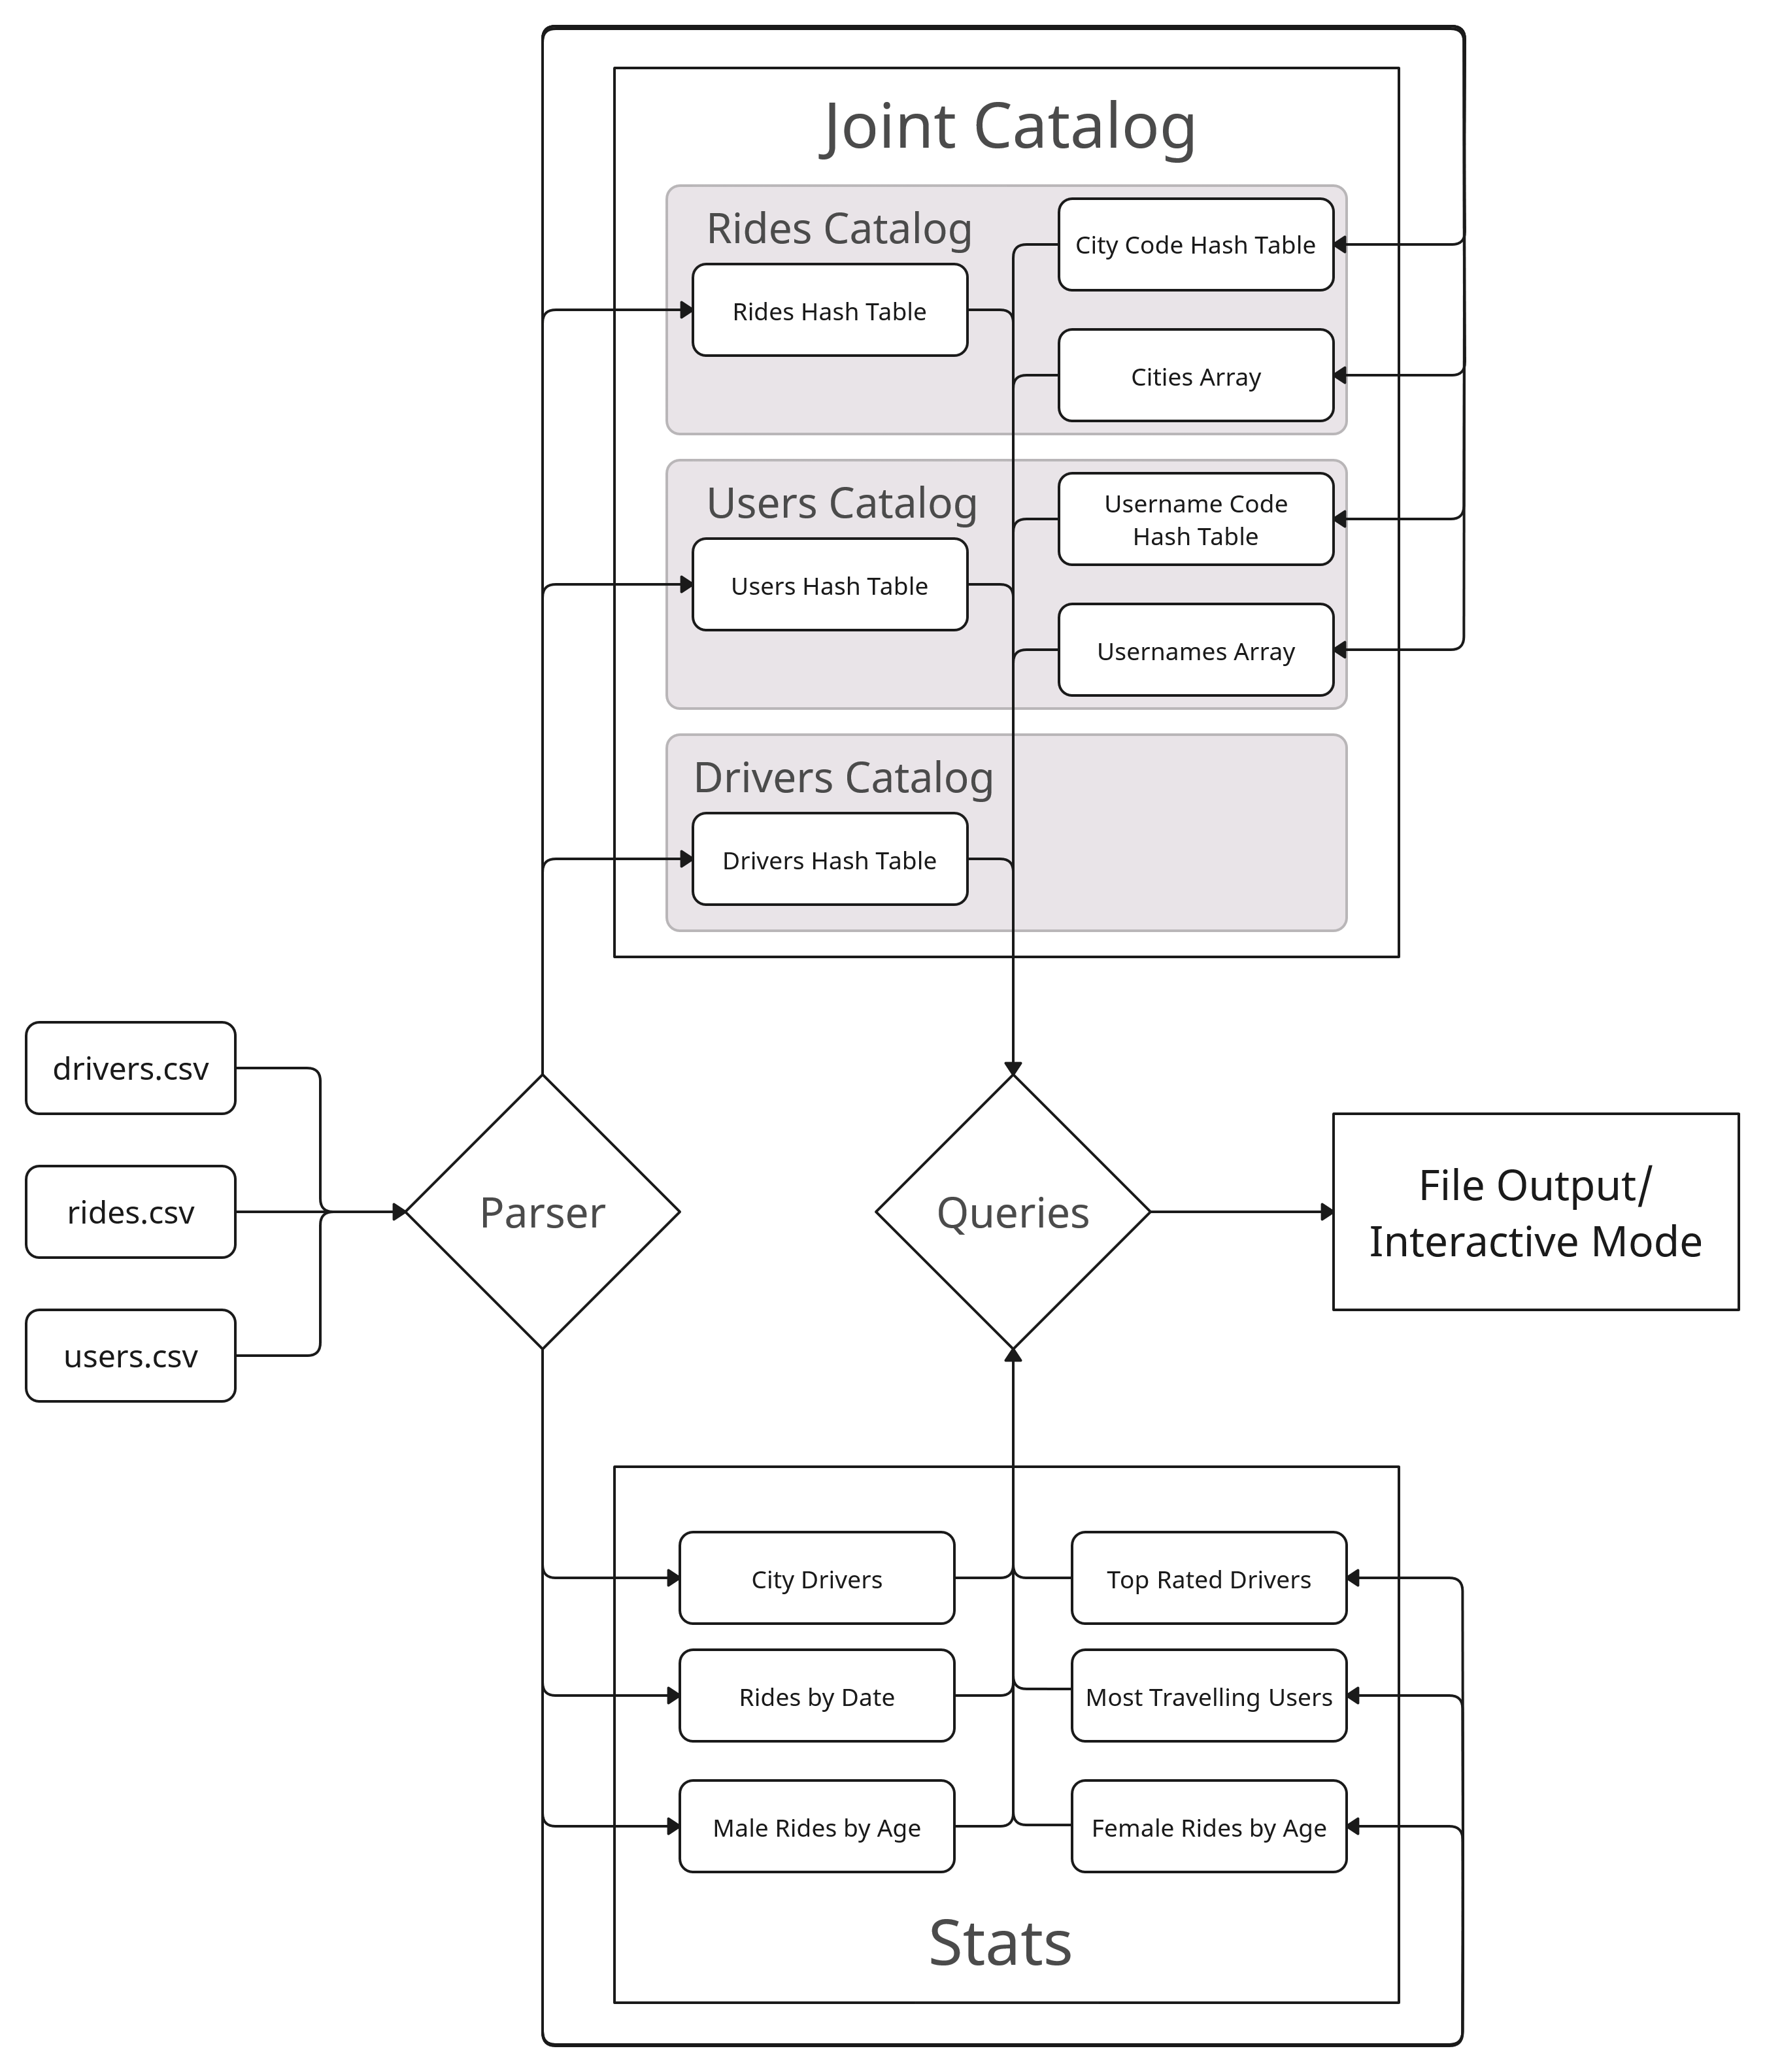
\includegraphics[scale = 0.155]{diagram1.png}
    \centering
    \caption{Diagrama da arquitetura na segunda fase}
    \end{figure} 
    
\newpage

    \chapter{Queries}
    
    \par Na primeira fase, tínhamos decidido focarmo-nos nas \textit{queries} 1,2 e 3, visto que foi as que consideramos mais simples de implementar. A única mudança que realizamos a estas \textit{queries} foi alterar a estrutura temporária de ordenação dos utilizadores na segunda e terceira \textit{queries} de uma \textit{linked list} para um \textit{array}, devido à maior eficiência de memória e rapidez. Nesta fase implementamos as restantes queries, ordenadas nesta secção pela estrutura auxiliar que utilizam:
    \subsubsection{City Drivers}
    \par \textbf{Query 4}: É nos fornecida a \textit{string} da cidade e precisamos calcular o \textit{"preço médio das viagens (sem considerar gorjetas) numa determinada cidade"}.
    Esta query é processada com ajuda da estrutura de estatísticas \textit{City Drivers}, que consiste num \textit{array} onde cada posição corresponde às estatísticas de cada cidade (segundo o código da mesma). Nessas estatísticas estão guardadas várias informações, mas as únicas relevantes para esta \textit{query} são o valor total gasto e o número de rides efetuadas nessa cidade. A divisão do primeiro com o segundo é então devolvida como a resposta.
    \par \textbf{Query 7}: É pedido para determinarmos o \textit{"top n condutores numa determinada cidade, ordenado pela avaliação média do condutor"}. Nesta \textit{query} voltamos a utilizar a estrutura de estatísticas anterior, mas utilizamos o array presente nessa estrutura, que armazena todos os condutores que realizaram viagens nessa cidade, juntamente com a avaliação total e o número de viagens realizadas pelo mesmo. Ao processar a \textit{query}, esses valores são ordenados pela avaliação média e de seguida devolvidos.
    \subsubsection{Rides by Date}
    \par \textbf{Query 5}: Calcular o \textit{"preço médio das viagens (sem considerar gorjetas) num dado intervalo de tempo"}. Esta \textit{query} faz uso da \textit{hash table Rides by Date}. Esta estrutura possui como chave uma data, e como valor um \textit{pointer} para uma \textit{struct}, denominada \texit{Rides of The Day}. Dentro dessa \textit{struct} podemos encontrar três valores, um que armazena o preço total de todas as viagens efetuadas nesse dia, um que armazena o número de viagens efetuadas nesse dia, e um \textit{array}, onde cada um dos elementos do mesmo representa todas as \textit{rides} efetuadas numa determinada cidade nesse dia. Todas as viagens efetuadas num determinado dia na cidade codificada com o número 2 estariam na terceira posição do \textit{array}, por exemplo. Abaixo apresentamos um esquema de um estado possível da estrutura, depois de dados serem inseridos na mesma, de modo a tornar a sua visualização mais simples:\\
    
    \begin{figure}[h]
    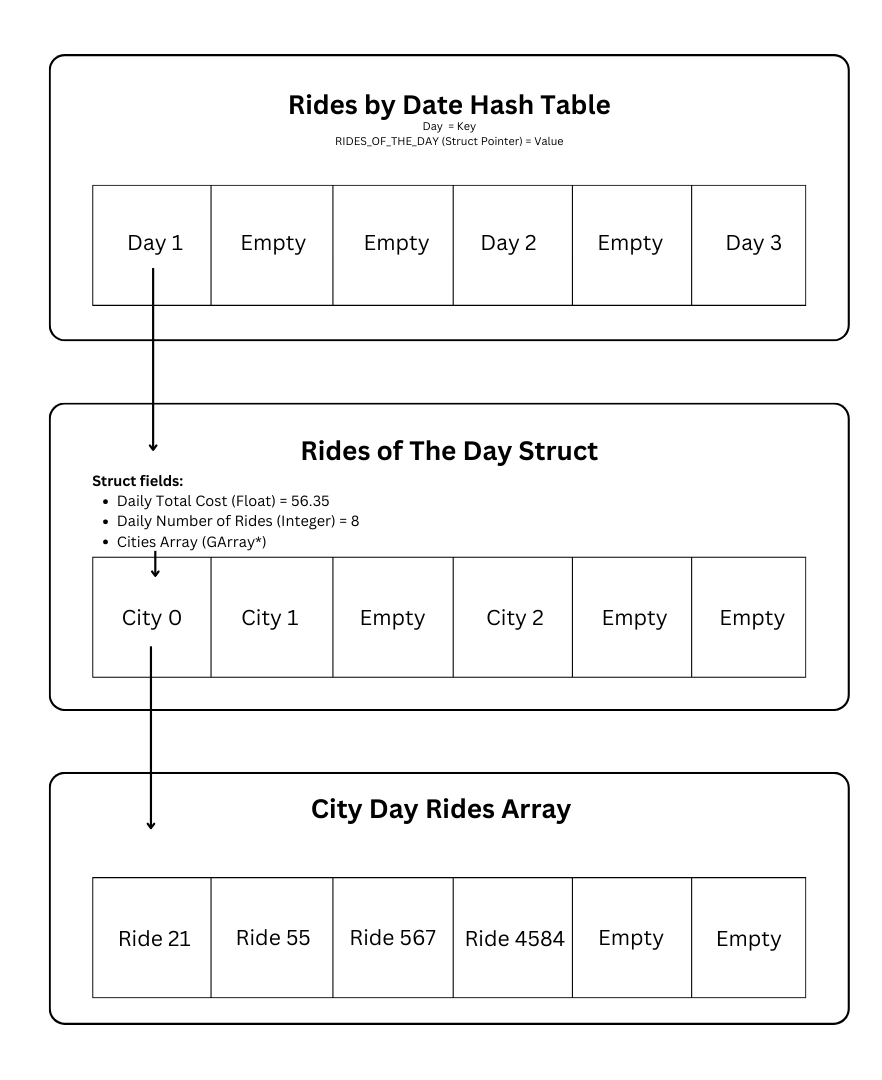
\includegraphics[scale = 0.45]{diagram2.png}
    \centering
    \caption{Diagrama de uma possível disposição da estrutura Rides by Date}
    \end{figure} 

    \par A \textit{query} 5 faz uso desta estrutura para procurar se existem viagens dentro do intervalo pedido (aproveitando o \textit{lookup} instantâneo das \textit{hash tables}), e adiciona custo e número de viagens total nesse dia ao total do intervalo que deseja procurar. No entanto, se o valor dos mesmos for -1, significa que o valor total de todas as viagens desse dia ainda não foi calculado. Esse valor será calculado pela \textit{query}, de modo a que \textit{queries} posteriores com sobreposições em intervalos de dias aproveitem esse valor já calculado em vez de o terem de recalcular de raiz. No final, a soma dos custos totais de todos os dias no intervalo é dividido pelo número de viagens realizadas em todos esses dias, obtendo assim a média do preço das viagens durante o intervalo indicado.
    
    \par \textbf{Query 6}: Esta \textit{query} é muito semelhante à anterior, mas pede-nos a distância média em vez do valor, e para além de também restringir os dados pertinentes a um intervalo de tempo, limita-se a ter em conta viagens em uma única cidade, fornecida pela \textit{query}. Esta query utiliza a mesma estrutura auxiliar da anterior, e limita-se a aceder a todos os dias dentro do intervalo, verificar se existem viagens realizadas nessa cidade, e adicionar as distâncias das mesmas a um total, tal como o número total de viagens realizadas. Depois de todos os dias no intervalo serem tidos em conta, a distância média é calculada e devolvida.
    \par \textbf{Query9}: É pedido para \textit{"listar as viagens nas quais o passageiro deu gorjeta, num certo intervalo de tempo, ordenadas pela distância percorrida"}. Esta \textit{query} faz também uso da estrutura de estatísticas \textit{Rides by Date}, percorrendo todos os dias dentro do intervalo e registando todas as viagens do mesmo num \textit{array} auxiliar. Finalmente essas \textit{rides} são ordenadas pelos critérios definidos e devolvidas.
    \subsubsection{Male/Female Rides by Date}
    \par \textbf{Query8}: \textit{"Listar todas as viagens nas quais o utilizador e o condutor são do género passado como parâmetro, e têm perfis com x ou mais anos. O output deverá ser ordenado de forma que as contas mais antigas apareçam primeiro."}. Dependendo do género fornecido como argumento, a estrutura de estatísticas \textit{Male/Female Rides by Age} é utilizada. As estruturas são iguais, mas separadas por género, e ambas registam todas as viagens onde o condutor e o utilizador possuem o mesmo género. O \textit{array} escolhido é simplesmente ordenado segundo as idades do utilizador e/ou condutor e devolvido.

\newpage

    \chapter{Otimizações}
    
    \par Após concluirmos todas as \textit{queries}, sentimos que a \textit{performance} do programa estava longe de ser ideal. O tempo de execução do \textit{dataset} grande aproximava-se de um minuto e meio no servidor da equipa docente e a memória estava quase nos 4 \textit{gigabytes}. Logo, apesar do tempo de execução não ser um critério específico de avaliação, tentamos reduzi-lo ao máximo. Tal apenas seria possível observando as nossas implementações originais e perceber quais eram os seus pontos fracos, alterando-os para soluções mais eficientes. Para isso, utilizamos muitas vezes ferramentas para análise de performance - nomeadamente, o \textit{gprof} e o \textit{callgrind}.
    \par A primeira das nossas ideias foi repensar a nossa implementação das datas. Até esse momento as datas estavam definidas como uma \textit{struct} com três inteiros, representando cada um deles o dia, mês e ano respetivamente, mas resolvemos alterá-lo para apenas um inteiro com o formato AAAAMMDD. Desta forma, para além de gastarmos um terço da memória com datas, a comparação entre datas passou a ser instantânea pela subtração, enquanto anteriormente era necessário comparar ano, em caso de igualdade o mês, e em caso de igualdade o dia. Esta otimização pode parecer simples, mas reduziu o tempo de execução do programa em quase três segundos. 
    \par A partir daí continuamos a otimizar o nosso programa, e conseguimos superar a nossa meta de 45 segundos. Atualmente, o programa consegue processar o maior \textit{dataset} em cerca de 40 segundos no \textit{website}. Abaixo encontra-se uma tabela com o nosso progresso em tempo de execução e utilização de memória, e as principais otimizações que foram feitas para obter esses tempos.
    
    \begin{tabular}{|c||p{1,5cm}|p{3cm}|}
    \hline
    Otimização & Tempo & Uso de RAM \\
    \hline
    Original (\textit{queries} todas implementadas) & 69,58s & 3,9GB \\
    \hline 
    Codificação das datas em apenas um inteiro & 66,72s & 3,45GB \\
    \hline
   	Codificação dos driver e ride ids num inteiro & 60,45s & 2,96GB\\
    \hline
   	Mudança de \textit{GList} para \textit{GArray} nas \textit{queries} 2 e 3 & 60,13s & 2,9GB \\
    \hline
    Utilização do \textit{qsort} nas funções de sort & 59,63s & 2,9GB\\
    \hline
    Introdução da validação do input & 63,87s & 2,95GB\\
    \hline
    Codificação da cidade num inteiro & 43,93s & 2,32GB\\
    \hline
    Mudança de \textit{GTree} para \textit{GArray} na \textit{query} 7 & 29,39s & 2,2GB\\
    \hline
    Estrutura \textit{Rides by Date mais complexa} (\textit{queries} 5 e 6) & 27,91s & 2,2GB\\
    \hline
    Substituição de \textit{sscanf} por funções mais eficientes & 23,85s & 2,2GB \\
    \hline
    Alteração das keys nas hash tables para \textit{pointers}	 & 21,3s & 1,565GB \\
    \hline
    \end{tabular}
    \caption{ \label{demo-table} \begin{center}\footnotesize Nota: O tempo foi obtido compilando e executando cada uma das otimizações 10 vezes, removendo o pior e o melhor resultado,  calculando a média dos 8 restantes. Pode-se ainda referir que foi medido numa máquina com um CPU Ryzen 7 5700U e 16GB de RAM.
    \end{center}} 

    \par Podemos assim concluir que o tempo de execução foi descendo à medida que implementamos mais otimizações, apenas aumentando quando implementamos  a verificação do input, visto que todos as entradas tiveram de ser verificadas, o que adicionou mais tarefas ao programa.
    

\newpage

    \chapter{Verificação de input}
    
    \par Esta componente do programa, apesar de simples, é crucial de modo a certificarmo-nos que o \textit{input} está correto, de modo a não causar problemas de dados inválidos ou vazios, resultando em \textit{queries} incorretas.
    \par A implementação destes requisitos, apesar de não muito complexa, tinha de ser eficiente de modo a não impactar seriamente a performance do programa. Inicialmente ponderamos utilizar \textit{regex} para verificar se o \textit{input} cumpria os formatos solicitados, tendo até implementado verificações para alguns campos, mas devido ao enorme tempo de compilação dos mesmos, resolvemos verificar os caracteres um a um, apenas utilizando a função \textit{sscanf} nas verificações mais complexas, mas que posteriormente também acabamos por substituir por verificações diretas, mais eficientes.

\newpage

    \chapter{Modo interativo}
    
     \par Um dos requisitos principais desta fase foi a implementação de um modo interativo, com interface gráfica no terminal. Recorremos à biblioteca \textit{ncurses} para tal, visto que esta facilita a criação de um modo gráfico e uniformiza e simplifica a nossa implementação. O modo gráfico é capaz de:
    
    \begin{itemize}
    \item Processar \textit{queries} e devolver os seus resultados;
    \item No caso dos resultados serem grandes demais para serem imprimidos no ecrã ao mesmo tempo, os resultados são paginados e o utilizador pode fazer "scroll" \space pelos mesmos;
    \item Um menu de ajuda, detalhando a função de cada \textit{query}.
    \end{itemize}
   
   	\par Um dos pontos fulcrais para o sucesso do modo interativo foi o desenvolvimento de uma espécie de biblioteca de componentes. Basicamente, componentes como menus, \textit{option switchers}, \textit{labels}, entre outros, estão definidos num módulo de componentes e podem ser utilizados por qualquer página do modo interativo, já que recebem \textit{propriedades} bastante modulares.

    \begin{figure}[h]
    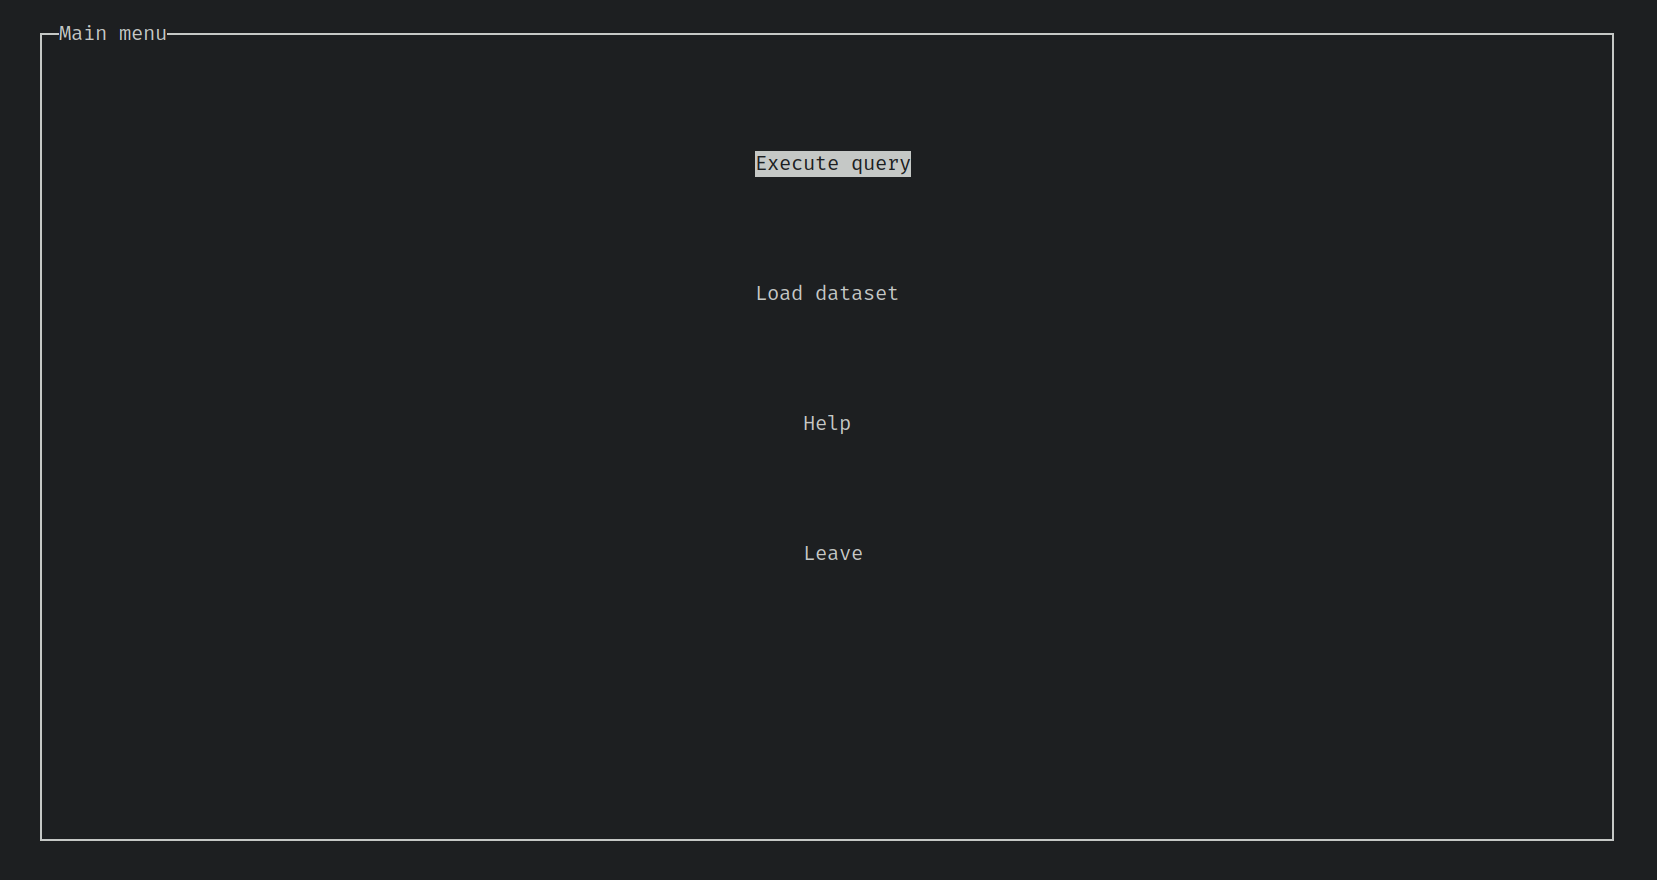
\includegraphics[scale = 0.25]{main_menu.png}
    \centering
    \caption{Menu principal, onde estão todas as funcionalidades do programa}
    \end{figure} 

    \begin{figure}[h]
    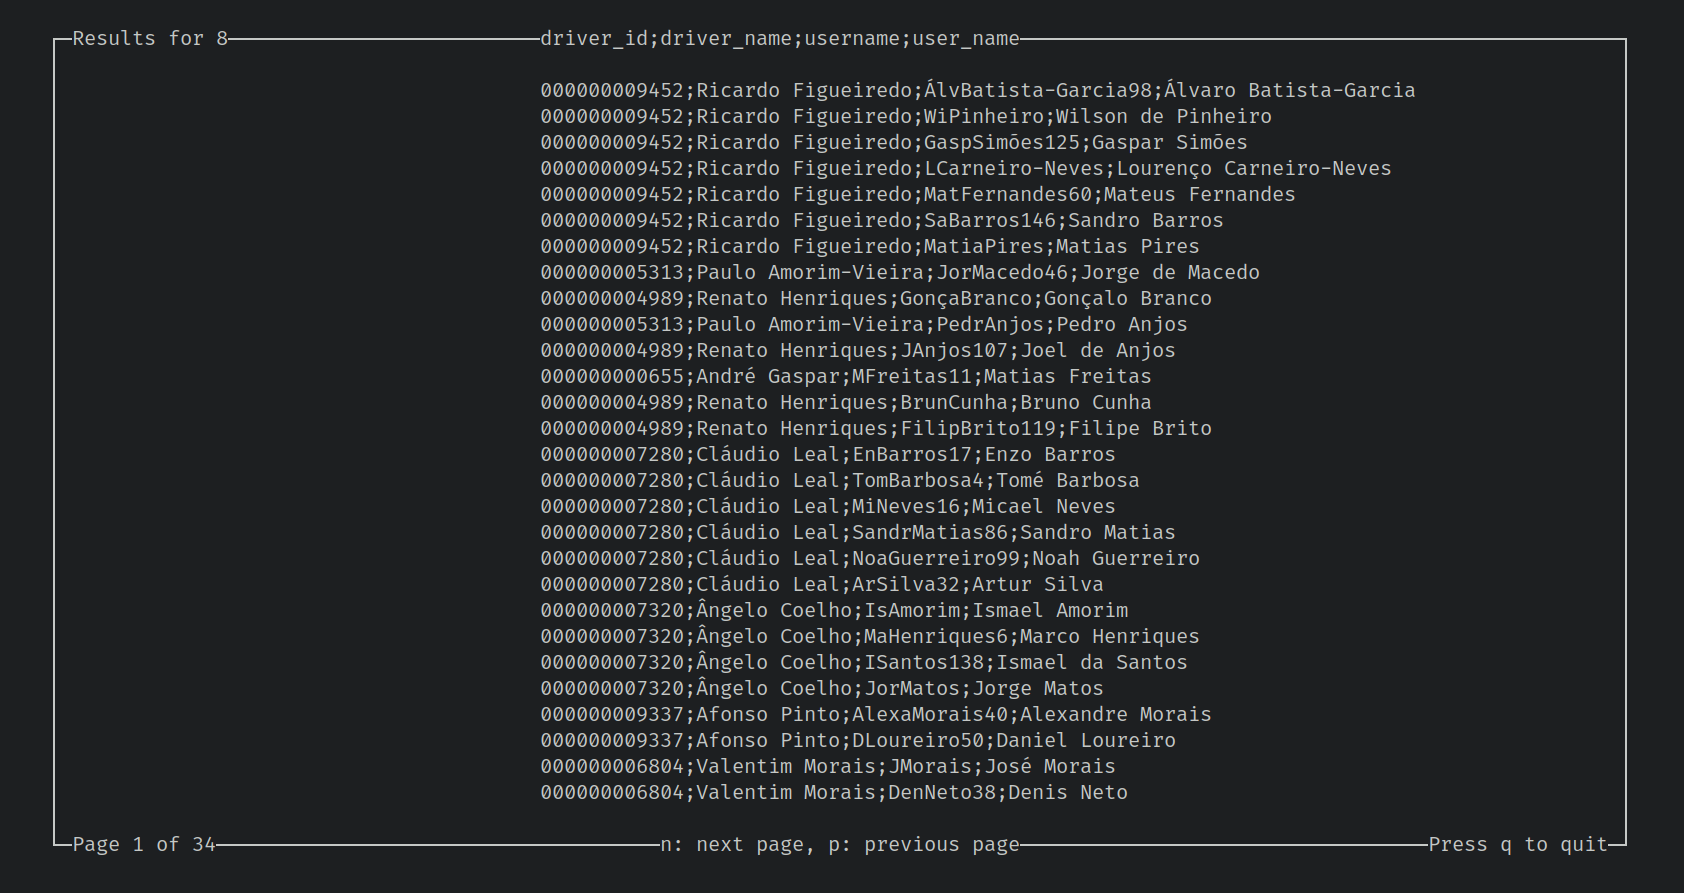
\includegraphics[scale = 0.25]{query_result.png}
    \centering
    \caption{Resultados de uma \textit{query} com muitas entradas, onde é possível passar para a próxima "página"  \space de resultados }
    \end{figure} 

\newpage

    \chapter{Dificuldades sentidas}

 	\par Nesta fase, apesar dos desafios serem de muito maior complexidade, como já tínhamos a arquitetura e ideia base de como iríamos estruturar o projeto, sentimo-nos mais organizados e preparados. No entanto, não quer dizer que não tenhamos encontrado dificuldades durante o desenvolvimento.
    \par Inicialmente, tivemos alguma dificuldade em implementar as estruturas auxiliares corretamente, visto que ainda não estávamos completamente confortáveis com a \textit{glib}, de onde utilizamos funções para criar estruturas, e visto que a documentação da mesma poderia ser mais clara em relação a algumas situações específicas.
    \par Também encontramos alguns entraves ao encapsulamento. Inicialmente pensávamos que o nosso programa estava completamente encapsulado, mas mais tarde percebemos que as nossas estruturas de dados estavam a ser diretamente acessados pelos módulos das estatísticas e das \textit{queries}, quebrando assim o encapsulamento. Resolvemos esse problema definindo funções dentro do módulo de cada estrutura. Além disso, existiu sempre alguma dificuldade associada à modularidade do programa. Temos pleno noção que algumas partes poderiam estar mais modulares, como, por exemplo, o módulo do output.
    \par Também existiu alguma dificuldade inicial em implementar verificação do \textit{input} pois encontramos um bug que foi difícil diagnosticar. A origem estava na função em que baseamos o nosso \textit{parser}, a \textit{strtok}, visto que esta reagia mal a campos vazios no \textit{input}, pois alocava um \textit{pointer}, portanto, ao tentarmos acessá-lo atingíamos um \textit{segfault}. Resolvemos este problema substituindo a \textit{strtok} pela \textit{strstr} e alterando o nosso \textit{parser} para a acomodar.

    
\newpage

    \chapter{Desempenho e testes}
    
    Neste capítulo iremos abordar o desempenho final do nosso programa e o módulo de testes que desenvolvemos para validar a correta implementação das \textit{queries}.
    Para testar a performance escolhemos o \textit{dataset} grande, sem erros, visto que o mesmo, com os seus testes acompanhantes, era o mais demorado, logo era o melhor a demonstrar diferenças de performance entre máquinas. 
    \par Para além de realizar apenas as 500 \textit{queries}, fizemos um versão alternativa onde realizamos um total de 2000 \textit{queries}, e registamos também o seu desempenho.
    \par Em baixo apresentamos os resultados do tempo de execução em três diferentes máquinas. \\
    
    \begin{tabular}{|c||p{3,5cm}|p{3,5cm}|p{3,75cm}|}
    \hline
    & Máquina 1 & Máquina 2 & Máquina 3 \\
    \hline
    CPU & Intel Core i5-8300H & Apple M1 & Ryzen 7 5700U \\
    \hline
    Cores/Threads & 4/8 & 8/8 & 8/16 \\
    \hline
    RAM & 16GB DDR4 2666 & 16GB DDR4 4266 & 16GB LPDDR4 4200 \\
    \hline
    Disco & 512GB SSD M.2 & 512 GB SSD M.2 & 512GB SSD M.2 \\
    \hline
    OS & Arch Linux & macOS Monterrey & Arch Linux \\
    \hline
    Compilador/Versão & gcc 12.2.1 & gcc 12.2.0 & gcc 12.2.1 \\
    \hline
    Pico de memória & 1,641GB & 1,641GB & 1,641GB \\
    \hline
    Tempo 500 \texit{queries} & 17,379s & 13,501s & 17,043s \\
    \hline
    Tempo 2000 \texit{queries} & 18,960s & 14,237s & 17,996s \\
    \hline
    \end{tabular}
    \caption{ \label{demo-table} \begin{center}\footnotesize Nota: O tempo foi obtido compilando e executando o programa 10 vezes, removendo o pior e o melhor resultado, e calculando a média dos 8 restantes.
    \end{center}} 
    
    \par É possível perceber que o tempo das 2000 queries é bastante próximo ao tempo das 500 queries. Isto deve-se principalmente ao sistema de \textit{caching} que desenvolvemos individualmente para cada \textit{query}. Além disso, deve-se também ao referido \textit{workload} inicial do programa.
 
    \par Em termos de memória, foi atingido um pico de 1641 \textit{megabytes} em cada uma das máquinas, algo pouco significante tendo em conta o tamanho dos dados inseridos e bem abaixo do limite de 4GB pedido pelos docentes. A nossa utilização de memória chegou a estar bem próxima do limite de 4GB, aquando da implementação de todas as \textit{queries}, mas devido às várias otimizações implementadas, já abordadas no capítulo 4, conseguimos reduzir esta utilização aproximadamente em 60\%.
    \par Já o módulo de testes faz vários tipos de testes todas as queries, com vários \textit{inputs}, medindo o tempo individual, total e a memória em pico. Este módulo é bastante útil para verificar se o programa funciona corretamente, sendo essencial para novas implementações ou manutenção do programa, pois é possível alguma mudança ter acidentalmente mudado o funcionamento do programa, e estes testes ajudam a diagnosticar tais problemas. O mesmo foi desenvolvido com recurso à \textit{framework} de testes da glib, que é bastante simples e intuitiva de implementar. Além disso, por necessidade própria, desenvolvemos outras formas de testar o nosso programa - desenvolvemos um script em bash que consegue rapidamente testar a diferença entre o conteúdo dos ficheiros entre duas pastas (bastante útil para comparar o resultado esperado, cedido pelos docentes, com o resultado obtido). Desenvolvemos também alguns actions no GitHub, nomeadamente para verificar a compilação, formatação e testar o nosso programa.
    
\newpage

    \chapter{Conclusão}
    
    \par Resumindo, apesar deste projeto e desta segunda fase, mais especificamente, serem um grande desafio, com muitos conceitos novos e de implementação complexa, sentimos, apesar de termos cometido alguns erros, estarmos à altura do desafio, em grande parte pelo nosso trabalho na primeira fase e as boas bases que desenvolvemos. Sentimos que melhoramos o nosso trabalho em relação à fase anterior em todos os aspetos, e que aplicamos corretamente os fundamentos base deste projeto, como a modularidade e encapsulamento, que pensamos serem conceitos fundamentais que qualquer engenheiro de software deveria ser capaz de aplicar.
\end{document}